
\chapter[The burst mode]{The burst mode of the mutant sodium channel}
\label{burst_chap}

We observed above that the effect of the $\Delta$KPQ mutation of the SCN5A
gene leading to a delayed sodium current can be modeled by increasing the
reaction rates from the inactivated state to the open state and to the
permissible state $C_{0}$. The model gave results at least qualitatively 
similar to the experimental data (see Figure \ref{NaM:mc}). 

A better-established way of
modeling the effect of the mutation is to introduce a so-called burst mode.
A simple Markov model including a burst mode is illustrated in Figure \ref{burst_prototype}, where the states of the burst mode
are indicated by $\ast$. Note that when the channel is in the burst mode,
there is no inactivated state and therefore the burst mode can be used to model the effect of impaired inactivation.
The reaction rates going from the burst mode to
the normal mode are given by $k^{u}$ (where $u$ stands for up) and the reaction rates from the normal mode
to the burst mode are given by $k^{d}$
(where $d$ stands for down). We assume $k^{d}<<k^{u}$, which means that, for the wild type, 
the probability of being in the burst mode is very small. The probability
of being in the burst mode increases with the mutation severity index $\mu$.
As usual, $\mu=1$ represents the wild type. In the wild type, a channel is basically never in the burst mode and therefore the channel inactivates as it should and no late sodium current is observed. In the mutant case, however, the probability of being in the burst mode is increased. Since there is no inactivated state in the burst mode, the channel fails to inactivate and therefore the probability of being in the open state is increased and therefore we observe a non-negligible late current. This will be illustrated in the numerical computations below.

\begin{figure}[ptb]
\begin{center}
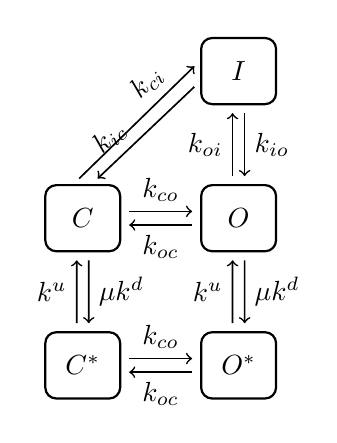
\begin{tikzpicture}[
   font=\sffamily,
   every matrix/.style={ampersand replacement=\&,column sep=1cm,row sep=1cm},
   state/.style={draw,thick,rounded corners,inner sep=.3cm},
   to/.style={->,semithick,shorten >=0.1cm,shorten <=0.1cm},
   Q/.style={->,semithick,sloped,pos=0.700000,shorten >=0.1cm,shorten <=0.1cm},  
   every node/.style={auto}]
\matrix{
\&\node[state] (I) {\parbox{10pt}{\centerline{$I$}}};\\
\node[state] (C) {\parbox{10pt}{\centerline{$C$}}};\&\node[state] (O) {\parbox{10pt}{\centerline{$O$}}};\\
\node[state] (C^{*}) {\parbox{10pt}{\centerline{$C^{*}$}}};\&\node[state] (O^{*}) {\parbox{10pt}{\centerline{$O^{*}$}}};\\
};
\draw[to]  (O^{*}.100) to node {$k^{u}$} (O.260);
\draw[to]  (O^{*}.190) to node {$k_{oc}$} (C^{*}.350);
\draw[to]  (O.280) to node {$\mu k^{d}$} (O^{*}.80);
\draw[to]  (O.100) to node {$k_{oi}$} (I.260);
\draw[to]  (O.190) to node {$k_{oc}$} (C.350);
\draw[to]  (I.280) to node {$k_{io}$} (O.80);
\draw[Q]  (I.195) to node {$k_{ic}$} (C.75);
\draw[to]  (C.10) to node {$k_{co}$} (O.170);
\draw[Q]  (C.105) to node {$k_{ci}$} (I.165);
\draw[to]  (C.280) to node {$\mu k^{d}$} (C^{*}.80);
\draw[to]  (C^{*}.10) to node {$k_{co}$} (O^{*}.170);
\draw[to]  (C^{*}.100) to node {$k^{u}$} (C.260);
\end{tikzpicture}
\end{center}
\caption{Prototypical model of a sodium channel including a burst mode. 
 The model consists of the states $O,I,$ and $C$ of the normal mode and $O^{*}$ and
$C^{*}$ of the burst mode (lower part). }
\label{burst_prototype}
\end{figure}



\section{Equilibrium probabilities}

We will start by considering the equilibrium states of the prototypical
model illustrated in Figure \ref{burst_prototype}. By following the usual steps
(see, e.g., page \pageref{9001}) we find
\begin{comment}
The equilibrium solutions are characterized by
the system of equations
\begin{align}
k_{io}i  &  =k_{oi}o,\text{ }k_{ci}c=k_{ic}i,\text{ }k_{co}c=k_{oc}o,\\
\mu k^{d}c  &  =k^{u}c^{\ast},\text{ }\mu k^{d}o=k^{u}o^{\ast}.
\end{align}
As usual, all variables can be expressed in terms of the open probability,
\begin{equation}
i=\frac{k_{oi}}{k_{io}}o,\text{ }c=\frac{k_{oc}}{k_{co}}o,\text{ }c^{\ast
}=\frac{\mu k^{d}}{k^{u}}\frac{k_{oc}}{k_{co}}o,\text{ }o^{\ast}=\frac{\mu
k^{d}}{k^{u}}o,
\end{equation}
and, since $o+i+c+c^{\ast}+o^{\ast}=1,$ we have
\begin{equation}
\left(  1+\frac{k_{oi}}{k_{io}}+\frac{k_{oc}}{k_{co}}+\frac{\mu k^{d}}{k^{u}
}\frac{k_{oc}}{k_{co}}+\frac{\mu k^{d}}{k^{u}}\right)  o=1
\end{equation}
and therefore
\end{comment}
 the equilibrium probabilities given by
\begin{align}
o  &  =\frac{1}{1+\frac{k_{oi}}{k_{io}}+\frac{k_{oc}}{k_{co}}+\frac{\mu k^{d}
}{k^{u}}\frac{k_{oc}}{k_{co}}+\frac{\mu k^{d}}{k^{u}}},\\
i  &  =\frac{\frac{k_{oi}}{k_{io}}}{1+\frac{k_{oi}}{k_{io}}+\frac{k_{oc}
}{k_{co}}+\frac{\mu k^{d}}{k^{u}}\frac{k_{oc}}{k_{co}}+\frac{\mu k^{d}}{k^{u}
}},\\
c  &  =\frac{\frac{k_{oc}}{k_{co}}}{1+\frac{k_{oi}}{k_{io}}+\frac{k_{oc}
}{k_{co}}+\frac{\mu k^{d}}{k^{u}}\frac{k_{oc}}{k_{co}}+\frac{\mu k^{d}}{k^{u}
}},\\
c^{\ast}  &  =\frac{\frac{k_{oc}}{k_{co}}\frac{\mu k^{d}}{k^{u}}}
{1+\frac{k_{oi}}{k_{io}}+\frac{k_{oc}}{k_{co}}+\frac{\mu k^{d}}{k^{u}}
\frac{k_{oc}}{k_{co}}+\frac{\mu k^{d}}{k^{u}}},\\
o^{\ast}  &  =\frac{\frac{\mu k^{d}}{k^{u}}}{1+\frac{k_{oi}}{k_{io}}
+\frac{k_{oc}}{k_{co}}+\frac{\mu k^{d}}{k^{u}}\frac{k_{oc}}{k_{co}}+\frac{\mu
k^{d}}{k^{u}}}.
\end{align}
Here, we observe that the equilibrium probability of being in the inactivated
state is clearly reduced as the mutation severity index is increased. This is
the effect we wanted, since inactivation is impaired in the
mutation and the effect is modeled by introducing a burst mode that lacks the
inactivated state. Second, we observe that the sum of the open probabilities
given by
\begin{equation}
o+o^{\ast}=\frac{1+\mu\frac{k^{d}}{k^{u}}}{1+\frac{k_{oi}}{k_{io}}
+\frac{k_{oc}}{k_{co}}+\mu\frac{k^{d}}{k^{u}}\frac{k_{oc}}{k_{co}}+\mu
\frac{k^{d}}{k^{u}}}
\end{equation}
is an increasing function of $\mu;$ in fact,
\begin{equation}
\frac{d}{d\mu}\left(  o+o^{\ast}\right)  =\frac{\frac{k^{d}}{k^{u}}
\frac{k_{oi}}{k_{io}}}{\left(  1+\frac{k_{oc}}{k_{co}}+\frac{k_{oi}}{k_{io}
}+\mu\frac{k^{d}}{k^{u}}\frac{k_{oc}}{k_{co}}+\mu\frac{k^{d}}{k^{u}}\right)
^{2}}>0.
\end{equation}
So the model has the two main properties we seek: The equilibrium
probability of being in the inactivated state is reduced and the open probability
is increased.

\bigskip

\section{The mean open time}

We observed above (see page \pageref{mot_many}) that the formula for the mean open time can also
be derived in the presence of several open states. If we generalize the
argument to also take into account the inactivated state, we find that the
mean open time of the Markov model illustrated in Figure \ref{burst_prototype} is given by
\begin{equation}
\tau_{o,\mu}=\frac{\mu k^{d}+k^{u}}{\mu k^{d}k_{oc}+k^{u}\left(  k_{oc}
+k_{oi}\right)  }
\end{equation}
and, since
\begin{equation}
\frac{d\tau_{o,\mu}}{d\mu}=\frac{k_{oi}k^{d}k^{u}}{\left(  k^{u}k_{oc}+k^{u}k_{oi}+\mu k_{oc}k^{d}\right)  ^{2}},
\end{equation}
the mean open time increases as a function of the mutation severity index.

%\K{zzz Skal man skifte slik fra $k_{oc}$ og $k_{oi}$ til $k_{co}$ og $k_{io}$
%n\r{a}r man deriverer?}

\bigskip

\section{An optimal theoretical open state blocker}

\begin{figure}[ptb]
\begin{center}
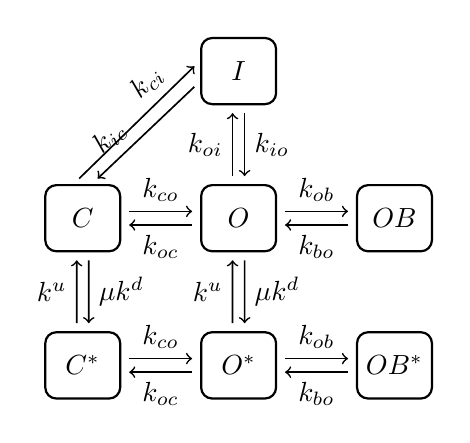
\begin{tikzpicture}[
   font=\sffamily,
   every matrix/.style={ampersand replacement=\&,column sep=1cm,row sep=1cm},
   state/.style={draw,thick,rounded corners,inner sep=.3cm},
   to/.style={->,semithick,shorten >=0.1cm,shorten <=0.1cm},
   Q/.style={->,semithick,sloped,pos=0.700000,shorten >=0.1cm,shorten <=0.1cm},  
   every node/.style={auto}]
\matrix{
\&\node[state] (I) {\parbox{10pt}{\centerline{$I$}}};\&\\
\node[state] (C) {\parbox{10pt}{\centerline{$C$}}};\&\node[state] (O) {\parbox{10pt}{\centerline{$O$}}};\&\node[state] (OB) {\parbox{10pt}{\centerline{$OB$}}};\\
\node[state] (C^{*}) {\parbox{10pt}{\centerline{$C^{*}$}}};\&\node[state] (O^{*}) {\parbox{10pt}{\centerline{$O^{*}$}}};\&\node[state] (OB^{*}) {\parbox{10pt}{\centerline{$OB^{*}$}}};\\
};
\draw[to]  (O^{*}.100) to node {$k^{u}$} (O.260);
\draw[to]  (O^{*}.10) to node {$k_{ob}$} (OB^{*}.170);
\draw[to]  (O^{*}.190) to node {$k_{oc}$} (C^{*}.350);
\draw[to]  (O.280) to node {$\mu k^{d}$} (O^{*}.80);
\draw[to]  (O.100) to node {$k_{oi}$} (I.260);
\draw[to]  (O.190) to node {$k_{oc}$} (C.350);
\draw[to]  (O.10) to node {$k_{ob}$} (OB.170);
\draw[to]  (I.280) to node {$k_{io}$} (O.80);
\draw[Q]  (I.195) to node {$k_{ic}$} (C.75);
\draw[to]  (C.10) to node {$k_{co}$} (O.170);
\draw[Q]  (C.105) to node {$k_{ci}$} (I.165);
\draw[to]  (C.280) to node {$\mu k^{d}$} (C^{*}.80);
\draw[to]  (OB.190) to node {$k_{bo}$} (O.350);
\draw[to]  (OB^{*}.190) to node {$k_{bo}$} (O^{*}.350);
\draw[to]  (C^{*}.10) to node {$k_{co}$} (O^{*}.170);
\draw[to]  (C^{*}.100) to node {$k^{u}$} (C.260);
\end{tikzpicture}
\end{center}
\caption{Prototypical model of a sodium channel including a burst mode and an open state blocker. 
 The model consists of the states $O,I,C,$ and $OB$ of the normal mode and $O^{*},C^{*},$ and $OB^*$ of the burst mode (lower part). 
 The states $OB$ and $OB^*$ represent the open blocker and we assume that the rates characterizing the blocker are the same in the normal and burst modes.}
\label{burst_prototype_drg}
\end{figure}


Our aim is now to define an open state drug that can repair both the
equilibrium open probability and the mean open time. The structure of the open
state blocker is given in Figure \ref{burst_prototype_drg} and the equilibrium total open probability is now
given by 
\begin{comment}
the following system of equations:
\begin{align*}
k_{io}i  &  =k_{oi}o,\text{ }k_{ci}c=k_{ic}i,\text{ }k_{co}c=k_{oc}o,\text{
}k_{bo}b=k_{ob}o,\\
\mu k^{d}c  &  =k^{u}c^{\ast},\text{ }\mu k^{d}o=k^{u}o^{\ast},\text{ }
k_{bo}b^{\ast}=k_{ob}o^{\ast}.
\end{align*}
Since
\begin{equation*}
i=\frac{k_{oi}}{k_{io}}o,\text{ }c=\frac{k_{oc}}{k_{co}}o,\text{ }c^{\ast
}=\frac{\mu k^{d}}{k^{u}}\frac{k_{oc}}{k_{co}}o,\text{ }o^{\ast}=\frac{\mu
k^{d}}{k^{u}}o,\text{ }b=\frac{k_{ob}}{k_{bo}}o,\text{ }b^{\ast}=\frac{k_{ob}
}{k_{bo}}\frac{\mu k^{d}}{k^{u}}o
\end{equation*}
and $o+i+c+c^{\ast}+o^{\ast}+b+b^{\ast}=1,$ 
we obtain the total open probability
\end{comment}
\begin{equation}
\left(  o+o^{\ast}\right)  _{\mu,d}=\frac{1+\mu\frac{k^{d}}{k^{u}}}{1+\frac
{k_{oi}}{k_{io}}+\frac{k_{oc}}{k_{co}}+\mu\frac{k^{d}}{k^{u}}\frac{k_{oc}
}{k_{co}}+\mu\frac{k^{d}}{k^{u}}+\frac{k_{ob}}{k_{bo}}\left(  1+\frac{\mu
k^{d}}{k^{u}}\right)  }. \label{o300}
\end{equation}
Furthermore, the mean open time is now given by
\begin{equation}
\tau_{o,\mu,d}=\frac{\mu k^{d}+k^{u}}{\mu k^{d}\left(  k_{oc}+k_{ob}\right)
+k^{u}\left(  k_{oc}+k_{oi}+k_{ob}\right)  }, \label{mot300}
\end{equation}
where the subscript $d$ is used to remind us that this concerns the case where
the theoretical drug has been applied.

\bigskip

The task at hand is now to tune the drug such that the equilibrium open
probability and the mean open time given by (ref{o300}) and
(ref{mot300}), respectively, are as close as possible to the equilibrium open
probability and the mean open time of the wild type. We regard the parameters
$k_{ob}$ and $k_{bo}$ as the unknowns and we want to solve the following
$2\times2$ system of equations:
\begin{align}
\frac{1+\mu\frac{k^{d}}{k^{u}}}{1+\frac{k_{oi}}{k_{io}}+\frac{k_{oc}}{k_{co}
}+\mu\frac{k^{d}}{k^{u}}\frac{k_{oc}}{k_{co}}+\mu\frac{k^{d}}{k^{u}}
+\frac{k_{ob}}{k_{bo}}\left(  1+\mu\frac{k^{d}}{k^{u}}\right)  }  &  =\frac
{1+\frac{k^{d}}{k^{u}}}{1+\frac{k_{oi}}{k_{io}}+\frac{k_{oc}}{k_{co}}+\frac{k^{d}}{k^{u}}
\frac{k_{oc}}{k_{co}}+\frac{k^{d}}{k^{u}}},\label{dr300}\\
\frac{\mu k^{d}+k^{u}}{\mu k^{d}\left(  k_{oc}+k_{ob}\right)  +k^{u}\left(
k_{oc}+k_{oi}+k_{ob}\right)  }  &  =\frac{k^{d}+k^{u}}{k^{d}k_{oc}
+k^{u}\left(  k_{oc}+k_{oi}\right)  }, \label{dr301}
\end{align}
where the latter equation determines the on rate, $k_{ob},$ of the drug,
\begin{equation}
k_{ob}=\left(  \mu-1\right)  \frac{k^{d}k^{u}k_{oi}}{\left(  k^{u}+\mu
k^{d}\right)  \left(  k^{u}+k^{d}\right)  }, \label{kob300}
\end{equation}
and we note that, in the case of $\mu=1,$ the  drug is completely turned off,
which is reasonable. Since $k_{ob}$ is known, the off rate of the drug can be
computed by solving (ref{dr300}) If we define
\begin{equation}
A=\frac{k_{ob}}{k_{bo}},
\end{equation}
we find from (ref{dr300})  
\begin{equation}
A=(\mu-1)\frac{k_{oi}}{k_{io}}  \frac{k^{u}k^{d}}{\left(  \mu k^{d}+k^{u}\right)  \left(  k^{d}
+k^{u}\right)  \label{Akbo}}
\end{equation}
and then the off rate of the drug is given by
\begin{equation}
k_{bo}=A^{-1}k_{ob}=k_{io} \label{kbo300}
\end{equation}
which is the same as we have in the prototypical model given in 
Figure \ref{MOT_mut_L:BICO_O}; see (\ref{mot_in_dr}) on page \pageref{mot_in_dr}.


\bigskip

\section{Numerical experiments}

\graytable{l}{
{|c|c|} \hline
$\mu$ & 20 \\ \hline
$k_u$ & 0.0001 $\rm{ms^{-1}}$\\ \hline
$k_d$ & 0.001 $\rm{ms^{-1}}$\\ \hline
$k_{ob}$ & 0.0286 $\rm{ms^{-1}}$\\ \hline
$k_{bo}$ &0.000824 $\rm{ms^{-1}}$\\ \hline
}{Values of the parameters used in the model in Figure \ref{burst_prototype_drg}.
The remaining rates  are as in Table \ref{markov_rates}.
\label{tab:burst_ob}}

The purpose of this section is to show how the burst mode can be used to represent impaired inactivation and how the theoretical drug derived above works. 

\subsection{Representation of the late sodium current using the burst mode model}

As discussed in Chapter \ref{simple_Na}, impaired inactivation leads to a late sodium current (see Figure \ref{NaM:mc}). Here, we will see that this effect can also be obtained using a Markov model of the form indicated in Figure \ref{burst_prototype}. In Figure \ref{NaB:current}, we repeat the computations reported in Figure \ref{NaM:mc}, using the Markov model of Figure \ref{burst_prototype}. The parameters used in this computation are given in Table \ref{tab:burst_ob}. We observe from Figure \ref{NaB:current} that $\mu=20$ seems to represent the late current of Figure \ref{NaM:mc} fairly well. 
 
 \subsection{The open state blocker repairs the effect of the mutation}

In Figure \ref{NaB:current}, we show the late current for the wild type, the mutant $\mu=20$, and the drug using the optimal open state blocker defined by (\ref{kob300}) and (\ref{kbo300}). We observe that the late current induced by the mutation is  repaired by the open state blocker. The statistics of the open probability density function (for the wild type, the mutant ($\mu=20$), and the mutant where the drug has been applied) are given in Table \ref{tab:burst_stat} and  
the corresponding probability density functions are shown in Figure \ref{NaB:ob}. Again we note that the open blocker repairs the main features of the solution.



FIGURE: [fig/NaB_current.pdf, width=500 frac=0.8] Currents computed using the Markov model illustrated in Figure \ref{burst_prototype_drg}. 
The simulations are based on averages of 10,000 runs. As expected, the open blocker asymptotically repairs the late current.  label{NaB:current}%FIGURE: [fig/NaB_current_zoom.pdf, width=500 frac=0.8] Just to illustrate that things work as expected, we might not want to use this one. label{NaB:current_zoom}FIGURE: [fig/NaB_ob.pdf, width=500 frac=0.8] Stationary probability density functions computed using the Markov model illustrated in Figure
\ref{burst_prototype_drg}. The open probability density function is given in the left panel and the probability density function of the sum of non-conducting states is given in the right panel. We observe that the open blocker repairs most parts of the probability density functions. label{NaB:ob}\begin{table}  \begin{center}
\begin{tabular}{|r|r|r|r|r|} \hline
$\mu$ & $\pi_o$ & $\pi_n$ & $E_o$ & $E_n$ \\ \hline
1 & 0.59 & 0.41 & 31.2 & -54.2 \\ \hline
20 & 0.96 & 0.04 & 33.1 & -52.8 \\ \hline
50 & 0.98 & 0.02 & 33.1 & -51.3 \\ \hline
100 & 0.99 & 0.01 & 33.2 & -49.8 \\ \hline
20+OB & 0.46 & 0.54 & 30.2 & -57.9 \\ \hline
\end{tabular} \end{center}
\caption{Statistics of the stationary probability density functions computed using the Markov model illustrated in Figure
\ref{burst_prototype_drg}. The subscript $o$ refers to open states and the subscript $n$ refers to non-conducting states.
 \label{tab:burst_stat}}
\end{table}



\section{A more sophisticated Markov model}
\label{sophisticated}

The Markov model presented in Figure \ref{burst_prototype} above has a structure that is a bit simpler than
the Markov model commonly used to model the sodium channel. A more common structure is given in 
Figure \ref{wtreac330}. This is the model we studied in Chapter \ref{simple_Na}. When a burst mode is added to it, the Markov model obtains the form illustrated in Figure \ref{burst}.


\begin{figure}[ptb]
\begin{center}
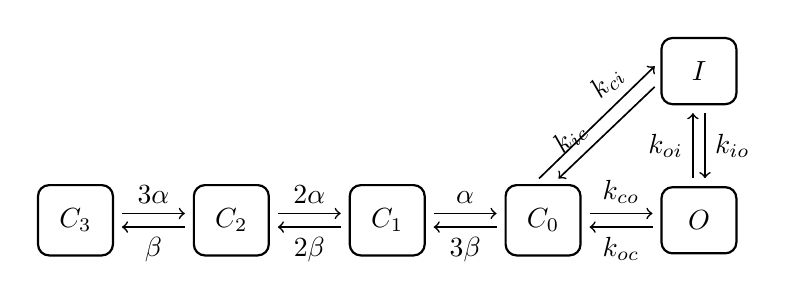
\begin{tikzpicture}[
   font=\sffamily,
   every matrix/.style={ampersand replacement=\&,column sep=1cm,row sep=1cm},
   state/.style={draw,thick,rounded corners,inner sep=.3cm},
   to/.style={->,semithick,shorten >=0.1cm,shorten <=0.1cm},
   Q/.style={->,semithick,sloped,pos=0.700000,shorten >=0.1cm,shorten <=0.1cm},  
   every node/.style={auto}]
\matrix{
\&\&\&\&\node[state] (I) {\parbox{10pt}{\centerline{$I$}}};\\
\node[state] (C_{3}) {\parbox{10pt}{\centerline{$C_{3}$}}};\&\node[state] (C_{2}) {\parbox{10pt}{\centerline{$C_{2}$}}};\&\node[state] (C_{1}) {\parbox{10pt}{\centerline{$C_{1}$}}};\&\node[state] (C_{0}) {\parbox{10pt}{\centerline{$C_{0}$}}};\&\node[state] (O) {\parbox{10pt}{\centerline{$O$}}};\\
};
\draw[to]  (O.100) to node {$k_{oi}$} (I.260);
\draw[to]  (O.190) to node {$k_{oc}$} (C_{0}.350);
\draw[to]  (I.280) to node {$k_{io}$} (O.80);
\draw[Q]  (I.195) to node {$k_{ic}$} (C_{0}.75);
\draw[to]  (C_{0}.10) to node {$k_{co}$} (O.170);
\draw[Q]  (C_{0}.105) to node {$k_{ci}$} (I.165);
\draw[to]  (C_{0}.190) to node {$3\beta$} (C_{1}.350);
\draw[to]  (C_{1}.10) to node {$\alpha$} (C_{0}.170);
\draw[to]  (C_{1}.190) to node {$2\beta$} (C_{2}.350);
\draw[to]  (C_{2}.10) to node {$2\alpha$} (C_{1}.170);
\draw[to]  (C_{2}.190) to node {$\beta$} (C_{3}.350);
\draw[to]  (C_{3}.10) to node {$3\alpha$} (C_{2}.170);
\end{tikzpicture}
\end{center}
\caption{Typical Markov model of a wild type sodium channel consisting of an open
state $(O)$, an inactivated state $(I)$, and four closed states $(C_{0}
,C_{1},C_{2}, \text{ and }C_{3})$. This model was analyzed in Chapter \ref{simple_Na}.}
\label{wtreac330}
\end{figure}



\begin{figure}[ptb]
\begin{center}
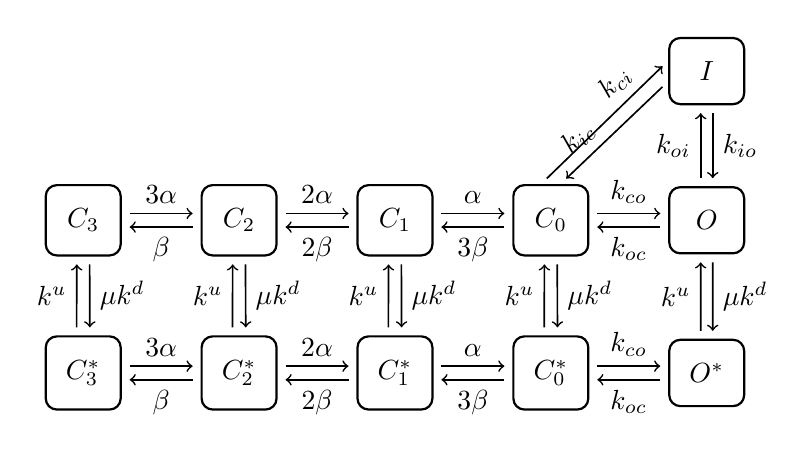
\begin{tikzpicture}[
   font=\sffamily,
   every matrix/.style={ampersand replacement=\&,column sep=1cm,row sep=1cm},
   state/.style={draw,thick,rounded corners,inner sep=.3cm},
   to/.style={->,semithick,shorten >=0.1cm,shorten <=0.1cm},
   Q/.style={->,semithick,sloped,pos=0.700000,shorten >=0.1cm,shorten <=0.1cm},  
   every node/.style={auto}]
\matrix{
\&\&\&\&\node[state] (I) {\parbox{10pt}{\centerline{$I$}}};\\
\node[state] (C_{3}) {\parbox{10pt}{\centerline{$C_{3}$}}};\&\node[state] (C_{2}) {\parbox{10pt}{\centerline{$C_{2}$}}};\&\node[state] (C_{1}) {\parbox{10pt}{\centerline{$C_{1}$}}};\&\node[state] (C_{0}) {\parbox{10pt}{\centerline{$C_{0}$}}};\&\node[state] (O) {\parbox{10pt}{\centerline{$O$}}};\\
\node[state] (C_{3}^{*}) {\parbox{10pt}{\centerline{$C_{3}^{*}$}}};\&\node[state] (C_{2}^{*}) {\parbox{10pt}{\centerline{$C_{2}^{*}$}}};\&\node[state] (C_{1}^{*}) {\parbox{10pt}{\centerline{$C_{1}^{*}$}}};\&\node[state] (C_{0}^{*}) {\parbox{10pt}{\centerline{$C_{0}^{*}$}}};\&\node[state] (O^{*}) {\parbox{10pt}{\centerline{$O^{*}$}}};\\
};
\draw[to]  (O^{*}.100) to node {$k^{u}$} (O.260);
\draw[to]  (O^{*}.190) to node {$k_{oc}$} (C_{0}^{*}.350);
\draw[to]  (O.280) to node {$\mu k^{d}$} (O^{*}.80);
\draw[to]  (O.100) to node {$k_{oi}$} (I.260);
\draw[to]  (O.190) to node {$k_{oc}$} (C_{0}.350);
\draw[to]  (I.280) to node {$k_{io}$} (O.80);
\draw[Q]  (I.195) to node {$k_{ic}$} (C_{0}.75);
\draw[to]  (C_{0}.10) to node {$k_{co}$} (O.170);
\draw[Q]  (C_{0}.105) to node {$k_{ci}$} (I.165);
\draw[to]  (C_{0}.190) to node {$3\beta$} (C_{1}.350);
\draw[to]  (C_{0}.280) to node {$\mu k^{d}$} (C_{0}^{*}.80);
\draw[to]  (C_{1}.10) to node {$\alpha$} (C_{0}.170);
\draw[to]  (C_{1}.190) to node {$2\beta$} (C_{2}.350);
\draw[to]  (C_{1}.280) to node {$\mu k^{d}$} (C_{1}^{*}.80);
\draw[to]  (C_{2}.10) to node {$2\alpha$} (C_{1}.170);
\draw[to]  (C_{2}.190) to node {$\beta$} (C_{3}.350);
\draw[to]  (C_{2}.280) to node {$\mu k^{d}$} (C_{2}^{*}.80);
\draw[to]  (C_{3}.10) to node {$3\alpha$} (C_{2}.170);
\draw[to]  (C_{3}.280) to node {$\mu k^{d}$} (C_{3}^{*}.80);
\draw[to]  (C_{0}^{*}.10) to node {$k_{co}$} (O^{*}.170);
\draw[to]  (C_{0}^{*}.100) to node {$k^{u}$} (C_{0}.260);
\draw[to]  (C_{0}^{*}.190) to node {$3\beta$} (C_{1}^{*}.350);
\draw[to]  (C_{1}^{*}.100) to node {$k^{u}$} (C_{1}.260);
\draw[to]  (C_{1}^{*}.10) to node {$\alpha$} (C_{0}^{*}.170);
\draw[to]  (C_{1}^{*}.190) to node {$2\beta$} (C_{2}^{*}.350);
\draw[to]  (C_{2}^{*}.100) to node {$k^{u}$} (C_{2}.260);
\draw[to]  (C_{2}^{*}.10) to node {$2\alpha$} (C_{1}^{*}.170);
\draw[to]  (C_{2}^{*}.190) to node {$\beta$} (C_{3}^{*}.350);
\draw[to]  (C_{3}^{*}.100) to node {$k^{u}$} (C_{3}.260);
\draw[to]  (C_{3}^{*}.10) to node {$3\alpha$} (C_{2}^{*}.170);
\end{tikzpicture}
\end{center}\caption{Markov model of the sodium channel. The model consists of the states
$O,I,C_{0},C_{1},C_{2},$ and $C_{3}$ of the normal mode and $O^{*},C^{*}
_{0},C^{*}_{1},C^{*}_{2},$ and $C^{*}_{3}$ of the burst mode (lower part). Note
that there is no inactivated state in the burst mode and that $\mu$ denotes
the mutation severity index. A larger value of $\mu$ increases the probability
of moving from the normal (upper) mode to the burst (lower) mode.}
\label{burst}
\end{figure}

To understand how the burst mode changes the properties of the model,
it is of interest to compute the equilibrium probabilities. 
%\begin{comment}
The equilibrium state of the model presented in Figure \ref{burst} is
characterized by the following system of equations:
\begin{equation}
\begin{array}
[c]{ccc}
k_{ci}c_{0}=k_{ic}i, & k_{oi}o=k_{io}i, & k_{co}c_{0}=k_{oc}o,\\
3\beta c_{0}=\alpha c_{1}, & 2\alpha c_{2}=2\beta c_{1}, & 3\alpha c_{3}=\beta c_{2},\\
k^{u}o^{\ast}=\mu k^{d}o, & k^{u}c_{0}^{\ast}=\mu k^{d}c_{0}, & k^{u}
c_{1}^{\ast}=\mu k^{d}c_{1},\\
k^{u}c_{2}^{\ast}=\mu k^{d}c_{2}, & k^{u}c_{3}^{\ast}=\mu k^{d}c_{3}. &
\end{array}
\label{ep1}
\end{equation}
It follows that
\begin{align*}
i &  =\frac{k_{oi}}{k_{io}}o,\text{ }c_{0}=\frac{k_{oc}}{k_{co}}o,\text{ }\\
c_{1} &  =\frac{3\beta}{\alpha}\frac{k_{oc}}{k_{co}}o,\text{ }c_{2}
=\frac{3\beta^{2}}{\alpha^{2}}\frac{k_{oc}}{k_{co}}o,\text{ }c_{3}=\frac
{\beta^{3}}{\alpha^{3}}\frac{k_{oc}}{k_{co}}o,\\
o^{\ast} &  =\mu\frac{k^{d}}{k^{u}}o,c_{0}^{\ast}=\mu\frac{k^{d}}{k^{u}}
\frac{k_{oc}}{k_{co}}o,c_{1}^{\ast}=\mu\frac{3\beta}{\alpha}\frac{k^{d}}
{k^{u}}\frac{k_{oc}}{k_{co}}o,\\
c_{2}^{\ast} &  =\mu\frac{3\beta^{2}}{\alpha^{2}}\frac{k^{d}}{k^{u}}
\frac{k_{oc}}{k_{co}}o,c_{3}^{\ast}=\mu\frac{\beta^{3}}{\alpha^{3}}\frac
{k^{d}}{k^{u}}\frac{k_{oc}}{k_{co}}o
\end{align*}
and, since the sum of the probabilities equals one, we have
%\end{comment}
\[
o\left(  \mu\right)  =\frac{1}{\frac{k_{oi}}{k_{io}}+\left(  1+\mu\frac{k^{d}
}{k^{u}}\right)  \left(  1+\frac{k_{oc}}{k_{co}}\left(  1+\beta/\alpha\right)
^{3}\right)  }
\]
and
\[
o\left(  \mu\right)  +o^{\ast}\left(  \mu\right)  =\frac{1+\mu\frac{k^{d}
}{k^{u}}}{\frac{k_{oi}}{k_{io}}+\left(  1+\mu\frac{k^{d}}{k^{u}}\right)
\left(  1+\frac{k_{oc}}{k_{co}}\left(  1+\beta/\alpha\right)  ^{3}\right)  }.
\]
Therefore,
\[
\frac{d}{d\mu}\left(  o\left(  \mu\right)  +o^{\ast}\left(  \mu\right)
\right)  =\frac{\frac{k_{oi}}{k_{io}}\frac{k^{d}}{k^{u}}}{\left(  \frac
{k_{oi}}{k_{io}}+\left(  1+\frac{k_{oc}}{k_{co}}\left(  1+\beta/\alpha\right)
^{3}\right)  \left(  1+\mu\frac{k^{d}}{k^{u}}\right)  \right)  ^{2}}>0,
\]
so the total open probability increases as the mutation severity index
$\mu$ increases. This will lead to a sustained sodium current characteristic
of the mutation under consideration. 

It is also interesting to see how the mutation severity index changes the
probability of being in the normal or burst mode. To understand
this, we define $b$ and $b^{\ast}$ as the sum of the probabilities in the
normal and burst modes, respectively. By using the equilibrium probabilities
derived above, we obtain
\[
\frac{b^{\ast}}{b}=\frac{o^{\ast}+c_{0}^{\ast}+c_{1}^{\ast}+c_{2}^{\ast}
+c_{3}^{\ast}}{o+c_{0}+c_{1}+c_{2}+c_{3}+i}=\mu\frac{k^{d}}{k^{u}}
\frac{1+\frac{k_{oc}}{k_{co}}\left(  1+\beta/\alpha\right)  ^{3}}
{\frac{k_{oi}}{k_{io}}+1+\frac{k_{oc}}{k_{co}}\left(  1+\beta/\alpha\right)
^{3}}
\]
and thus the probability of being in the burst mode increases as the mutation
severity index increases.

\bigskip

\section[Numerical experiments; burst mode]{Numerical experiments illustrating the effect of the burst mode}

\graytable{l}{
{|c|c|} \hline
$\mu$ & 1,10,30,100 \\ \hline
$k_u$ & 0.1 $\rm{ms^{-1}}$\\ \hline
$k_d$ & 0.01 $\rm{ms^{-1}}$\\ \hline
%$k_{ob}$ &  0.2196 $\rm{ms^{-1}}$\\ \hline
%$k_{bo}$ &0.0001578 $\rm{ms^{-1}}$\\ \hline
}{Values of the parameters used in the model in Figure \ref{burst}.
%\ref{burstdrg}.
The remaining rates  are as in Table \ref{markov_rates} on page \pageref{markov_rates}. \label{tab:burst_param}
}


The effect of increasing the mutation severity index of the Markov model given in Figure \ref{burst} is shown in
 Figure \ref{NaB:pdf3} using the parameters given in Table \ref{tab:burst_param}.
  %In the computations we use the parameters $k_u=0.1, k_d = 0.01$ and the mutation severity index is $\mu=1,10,30,100$ where $\mu=1$ (solid line) represents the wild type. 
 The associated currents are shown in Figure
 \ref{NaB:mc} and we note that when the mutation severity index increases, there is a significant late sodium current.
 
FIGURE: [fig/NaB_pdf3.pdf, width=500 frac=0.8]  The probability density functions of the open, closed, and inactivated states for the
burst mode model. The mutation severity index is given by $\mu=10,$ $30,$ and $100$ and the black line represents the wild type.
Note that we only show solutions for the values of the transmembrane potential where the solutions differ as a result of the mutations. label{NaB:pdf3}%FIGURE: [fig/NaB_mc.pdf, width=500 frac=0.8] \G{Top trace is WT, the other ones MT, with the lowest corresponding to $\mu=100$.} 
%Current from the burst model. Stronger mutations leads to slower closing of the channel. label{NaB:mc}
\begin{figure}[p]\centering
\vbox{
\includegraphics[width=0.9\linewidth]{NaB/mc.pdf}
\includegraphics[width=0.7\linewidth]{NaM/Bennet.png}
}
\caption{Currents computed using the Markov model including the burst mode (see Figure \ref{burst}). Top panel: Current for $\mu=1,$ $10,$ $30,$ $100$. Each trace is an average of 10,000 Monte Carlo runs and the current is computed by  $I=g_{Na} P_o (v-V_{Na})$, with the transmembrane potential at $v=0$ mV. The currents are normalized so that the wild type current peaks at -1. Here $V_{Na} = 45$ mV and $g_{Na} = 1$ mS:$\mbox{cm}^2$.  The lower figures are from Bennett et al. \cite{Bennett1995}.\label{NaB/mc}}
\end{figure}


%\begin{table}  \begin{center}
%\begin{tabular}{|r|r|r|r|r|r|r|} \hline
%$\mu$ & $\pi_o$ & $\pi_c$ & $\pi_i$ & $\rho_o$ & $\rho_c$ & $\rho_i$ \\ \hline
%1 & 0.00006 & 0.99961 & 0.00033 & -53.2 & -84.9 & -73.4 \\ \hline
%10 & 0.00008 & 0.99967 & 0.00024 & -26.1 & -84.9 & -67.5 \\ \hline
%30 & 0.00012 & 0.99969 & 0.00019 & -8.3 & -84.9 & -61.0 \\ \hline
%100 & 0.00022 & 0.99963 & 0.00015 & 10.5 & -84.9 & -54.2 \\ \hline
%\end{tabular} \end{center}
%\caption{ Expected values of the transmembrane potential for open, closed or inactivated
%states for increasing values of the mutation severity index $\mu$.} \label{tab:burst}
%\end{table}
\begin{table}  \begin{center}
\begin{tabular}{|r|r|r|r|r|} \hline
$\mu$ & $1000 \times \pi_o$ & $\pi_n$ & $E_o$ & $E_c$ \\ \hline
1 & 0.05738 &  0.99994 & -53.2 & -84.9 \\ \hline
10 & 0.08435 & 0.99992 & -26.1 & -84.9 \\ \hline
30 & 0.12109 & 0.99983 & -8.3 & -84.9 \\ \hline
100 & 0.22305 & 0.99978 & 10.5 & -84.9 \\ \hline
30+OB & 0.05490&0.99995 & -57.0 & -84.9 \\ \hline
\end{tabular} \end{center}
\caption{Probabilities and expected values of the transmembrane potential for open and non-conducting states for increasing values of the mutation severity index $\mu$.} \label{tab:burst}
\end{table}


%xxx Glenn xxx: repeat experiments of the previous model. That is repeat figure 11.3, table 11.2, figure 11.4.



\section[Theoretical drug for the burst mode model]{A theoretical drug for the
mutation represented by the burst mode}

 In the simplified Markov model presented in Figure \ref{burst_prototype} above, we saw
that an open blocker was able to repair the effect of the mutation.
Now the Markov model is extended (see Figure \ref{burst}), but it is reasonable to
believe that an open blocker is still the best alternative, since both the open
probability and the mean open time are affected by the mutation. We consider
the Markov model given in Figure \ref{burstdrg}, where an open blocker is added to both
the open states of the Markov model given in Figure \ref{burst}. 
\begin{comment}
The equilibrium state
of the Markov model given in Figure \ref{burstdrg} is characterized by
\begin{equation}
\begin{array}
[c]{ccc}
k_{ci}c_{0}=k_{ic}i, & k_{oi}o=k_{io}i, & k_{co}c_{0}=k_{oc}o,\\
3\beta c_{0}=\alpha c_{1}, & 2\alpha c_{2}=2\beta c_{1}, & 3\alpha c_{3}=\beta
c_{2},\\
k^{u}o^{\ast}=\mu k^{d}o, & k^{u}c_{0}^{\ast}=\mu k^{d}c_{0}, & k^{u}
c_{1}^{\ast}=\mu k^{d}c_{1},\\
k^{u}c_{2}^{\ast}=\mu k^{d}c_{2}, & k^{u}c_{3}^{\ast}=\mu k^{d}c_{3}, & \\
k_{ob}o=k_{bo}b, & k_{ob}o^{\ast}=k_{bo}b^{\ast}. &
\end{array}
\end{equation}
\end{comment}
By following our usual procedure, we find that
\begin{comment}
\begin{align*}
i &  =\frac{k_{oi}}{k_{io}}o,\text{ }c_{0}=\frac{k_{oc}}{k_{co}}o,\text{ }\\
c_{1} &  =\frac{3\beta}{\alpha}\frac{k_{oc}}{k_{co}}o,\text{ }c_{2}
=\frac{3\beta^{2}}{\alpha^{2}}\frac{k_{oc}}{k_{co}}o,\text{ }c_{3}=\frac
{\beta^{3}}{\alpha^{3}}\frac{k_{oc}}{k_{co}}o,\\
o^{\ast} &  =\mu\frac{k^{d}}{k^{u}}o,c_{0}^{\ast}=\mu\frac{k^{d}}{k^{u}}
\frac{k_{oc}}{k_{co}}o,c_{1}^{\ast}=\mu\frac{3\beta}{\alpha}\frac{k^{d}}
{k^{u}}\frac{k_{oc}}{k_{co}}o,\\
c_{2}^{\ast} &  =\mu\frac{3\beta^{2}}{\alpha^{2}}\frac{k^{d}}{k^{u}}
\frac{k_{oc}}{k_{co}}o,c_{3}^{\ast}=\mu\frac{\beta^{3}}{\alpha^{3}}\frac
{k^{d}}{k^{u}}\frac{k_{oc}}{k_{co}}o,\\
b &  =\frac{k_{ob}}{k_{bo}}o,b^{\ast}=\mu\frac{k_{ob}}{k_{bo}}\frac{k^{d}
}{k^{u}}o,
\end{align*}
\newline and, since the sum of the probabilities equals one, we have
\end{comment}
\[
\left(  o+o^{\ast}\right)  _{\mu,d}=\frac{1+\mu\frac{k^{d}}{k^{u}}}
{\frac{k_{ob}}{k_{bo}}\left(  1+\mu\frac{k^{d}}{k^{u}}\right)  +\frac{k_{oi}
}{k_{io}}+\left(  1+\mu\frac{k^{d}}{k^{u}}\right)  \left(  1+\frac{k_{oc}
}{k_{co}}\left(  1+\beta/\alpha\right)  ^{3}\right)  }.
\]
The associated mean open time is given by
\begin{equation}
\tau_{o,\mu,d}=\frac{\mu k^{d}+k^{u}}{\mu k^{d}\left(  k_{oc}+k_{ob}\right)
+k^{u}\left(  k_{oc}+k_{oi}+k_{ob}\right)  }.
\end{equation}
We now want to tune the drug characterized by the two parameters $k_{ob}$
and $k_{bo}$ such that
\[
\left(  o+o^{\ast}\right)  _{\mu,d}\approx\left(  o+o^{\ast}\right)  _{wt}
\]
and
\[
\tau_{o,\mu,d}\approx\tau_{o,wt},
\]
where the subscript {\it wt} denotes wild type values. As above, we have two equations
for the two unknowns  $k_{ob}$ and $k_{bo}$ and the solution is given by
\begin{equation}
k_{ob}=\left(  \mu-1\right)  \frac{k^{d}k^{u}k_{oi}}{\left(  k^{u}+\mu
k^{d}\right)  \left(  k^{u}+k^{d}\right)  } \label{na_drug_ob}
\end{equation}
and
\begin{equation}
k_{bo}=A^{-1}k_{ob},
\end{equation}
where
\begin{equation}
A=\frac{k_{oi}}{k_{io}}k^{u}k^{d}\frac{\mu-1}{\left(  \mu k^{d}+k^{u}\right)
\left(  k^{d}+k^{u}\right)  }.
\end{equation}
So we obtain
\begin{equation}
k_{bo}=k_{io}. \label{na_drug_bo}
\end{equation}
We note that the formulas for the optimal open blocker for the Markov model
given in Figure \ref{burstdrg} are exactly the same as for the open blocker of the prototype Markov
model given in Figure \ref{burst_prototype_drg}.


\begin{figure}[ptb]
\begin{center}
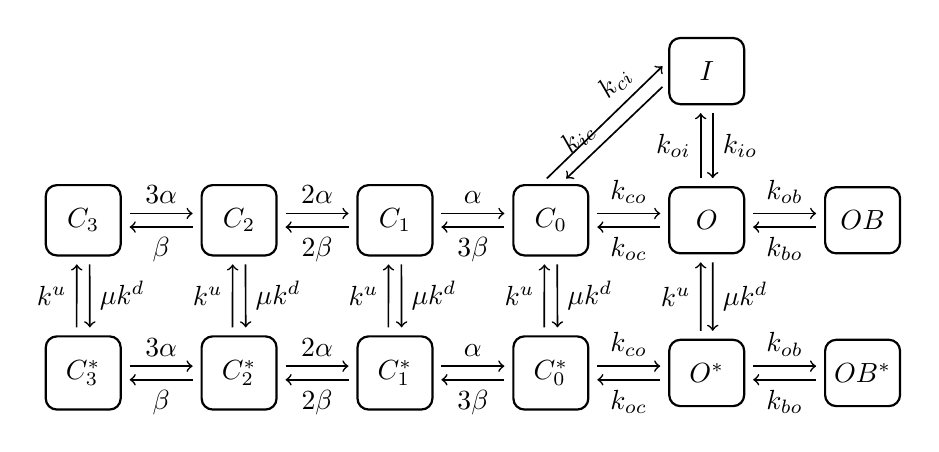
\begin{tikzpicture}[
   font=\sffamily,
   every matrix/.style={ampersand replacement=\&,column sep=1cm,row sep=1cm},
   state/.style={draw,thick,rounded corners,inner sep=.3cm},
   to/.style={->,semithick,shorten >=0.1cm,shorten <=0.1cm},
   Q/.style={->,semithick,sloped,pos=0.700000,shorten >=0.1cm,shorten <=0.1cm},  
   every node/.style={auto}]
\matrix{
\&\&\&\&\node[state] (I) {\parbox{10pt}{\centerline{$I$}}};\&\\
\node[state] (C_{3}) {\parbox{10pt}{\centerline{$C_{3}$}}};\&\node[state] (C_{2}) {\parbox{10pt}{\centerline{$C_{2}$}}};\&\node[state] (C_{1}) {\parbox{10pt}{\centerline{$C_{1}$}}};\&\node[state] (C_{0}) {\parbox{10pt}{\centerline{$C_{0}$}}};\&\node[state] (O) {\parbox{10pt}{\centerline{$O$}}};\&\node[state] (OB) {\parbox{10pt}{\centerline{$OB$}}};\\
\node[state] (C_{3}^{*}) {\parbox{10pt}{\centerline{$C_{3}^{*}$}}};\&\node[state] (C_{2}^{*}) {\parbox{10pt}{\centerline{$C_{2}^{*}$}}};\&\node[state] (C_{1}^{*}) {\parbox{10pt}{\centerline{$C_{1}^{*}$}}};\&\node[state] (C_{0}^{*}) {\parbox{10pt}{\centerline{$C_{0}^{*}$}}};\&\node[state] (O^{*}) {\parbox{10pt}{\centerline{$O^{*}$}}};\&\node[state] (OB^{*}) {\parbox{10pt}{\centerline{$OB^{*}$}}};\\
};
\draw[to]  (O^{*}.100) to node {$k^{u}$} (O.260);
\draw[to]  (O^{*}.10) to node {$k_{ob}$} (OB^{*}.170);
\draw[to]  (O^{*}.190) to node {$k_{oc}$} (C_{0}^{*}.350);
\draw[to]  (O.280) to node {$\mu k^{d}$} (O^{*}.80);
\draw[to]  (O.100) to node {$k_{oi}$} (I.260);
\draw[to]  (O.190) to node {$k_{oc}$} (C_{0}.350);
\draw[to]  (O.10) to node {$k_{ob}$} (OB.170);
\draw[to]  (I.280) to node {$k_{io}$} (O.80);
\draw[Q]  (I.195) to node {$k_{ic}$} (C_{0}.75);
\draw[to]  (C_{0}.10) to node {$k_{co}$} (O.170);
\draw[Q]  (C_{0}.105) to node {$k_{ci}$} (I.165);
\draw[to]  (C_{0}.190) to node {$3\beta$} (C_{1}.350);
\draw[to]  (C_{0}.280) to node {$\mu k^{d}$} (C_{0}^{*}.80);
\draw[to]  (C_{1}.10) to node {$\alpha$} (C_{0}.170);
\draw[to]  (C_{1}.190) to node {$2\beta$} (C_{2}.350);
\draw[to]  (C_{1}.280) to node {$\mu k^{d}$} (C_{1}^{*}.80);
\draw[to]  (C_{2}.10) to node {$2\alpha$} (C_{1}.170);
\draw[to]  (C_{2}.190) to node {$\beta$} (C_{3}.350);
\draw[to]  (C_{2}.280) to node {$\mu k^{d}$} (C_{2}^{*}.80);
\draw[to]  (C_{3}.10) to node {$3\alpha$} (C_{2}.170);
\draw[to]  (C_{3}.280) to node {$\mu k^{d}$} (C_{3}^{*}.80);
\draw[to]  (OB.190) to node {$k_{bo}$} (O.350);
\draw[to]  (OB^{*}.190) to node {$k_{bo}$} (O^{*}.350);
\draw[to]  (C_{0}^{*}.10) to node {$k_{co}$} (O^{*}.170);
\draw[to]  (C_{0}^{*}.100) to node {$k^{u}$} (C_{0}.260);
\draw[to]  (C_{0}^{*}.190) to node {$3\beta$} (C_{1}^{*}.350);
\draw[to]  (C_{1}^{*}.100) to node {$k^{u}$} (C_{1}.260);
\draw[to]  (C_{1}^{*}.10) to node {$\alpha$} (C_{0}^{*}.170);
\draw[to]  (C_{1}^{*}.190) to node {$2\beta$} (C_{2}^{*}.350);
\draw[to]  (C_{2}^{*}.100) to node {$k^{u}$} (C_{2}.260);
\draw[to]  (C_{2}^{*}.10) to node {$2\alpha$} (C_{1}^{*}.170);
\draw[to]  (C_{2}^{*}.190) to node {$\beta$} (C_{3}^{*}.350);
\draw[to]  (C_{3}^{*}.100) to node {$k^{u}$} (C_{3}.260);
\draw[to]  (C_{3}^{*}.10) to node {$3\alpha$} (C_{2}^{*}.170);
\end{tikzpicture}
\end{center}
\caption{Markov model of the mutant sodium channel with a blocker associated
with the open states. The model consists of the states $O,I,OB,C_{0}
,C_{1},C_{2},$ and $C_{3}$ of the normal mode and $OB^*,O^{*},C^{*}_{0},C^{*}
_{1},C^{*}_{2},$ and $C^{*}_{3}$ of the burst mode (lower part). The drug is
characterized by the two parameters $k_{bo}$ and $k_{ob}$.}
\label{burstdrg}
\end{figure}

\newpage

%\subsection{Numerical experiments}
%\graytable{l}{
%{|c|c|} \hline
%$\mu$ & 30\\ \hline
%$k_{ob}$ &  0.2196 $\rm{ms^{-1}}$\\ \hline
%$k_{bo}$ &0.0001578 $\rm{ms^{-1}}$\\ \hline
%}{Values of the parameters used in the model in Figure \ref{burstdrg}.
%%\ref{burstdrg}. 
%The remaining rates are as in Table \ref{tab:burst_param}.
%}


In Figure \ref{NaB:pdf3_d}, we show the probability density functions of the wild type, the mutant (using $\mu=30$), and
the mutant case where the optimal open blocker is applied. The blocker repairs the effect of the mutation and the same effect is seen in Figure \ref{NaB:mc_d} where the currents are given; the open blocker removes the late sodium current.


FIGURE: [fig/NaB_pdf3_d.pdf, width=500 frac=0.8] Probability density functions for the wild type, the mutant ($\mu=30$), and the mutant in the presence of the open blocker. The subscripts $o$ and $n$ refer to open and non-conduction states, respectively, where the states are shown in  Figure \ref{burstdrg}.}
\fig{NaB/mc_d.pdf}{Currents computed using the Markov model given in Figure \ref{burstdrg}
for the wild type, the mutant ($\mu=30$), and the mutant in the presence of the open blocker. label{NaB:pdf3_d}\clearpage

\section{Notes}
\label{notesburst}

\begin{enumerate}
\item The burst mode is discussed by Bennett et al. \cite{Bennett1995} and modeled
in the paper by Clancy and Rudy \cite{Clancy1999}.
\item The form of the model illustrated in Figure \ref{burst} is taken from Clancy and
Rudy \cite{Clancy1999}, but the functions and parameters of the model are not
taken from their paper.
\item As mentioned above, the introduction of a burst mode is a convenient way of modeling the effect of certain mutations. The notion that gating may enter various modes has been considerably extended and studied in the papers by Chakrapani et al. \cite{ Chakrapani2007a, Chakrapani2007b, Chakrapani2011} and by Ionescu et al. \cite{Ionescu2007}. In the recent paper by Siekmann et al \cite{Siekmann2014} the concept of modal gating is studied and a method for detecting mode changes based on single channel data is developed.
\end{enumerate}
